\section{Architectural Description}

\subsection{Overview}
	The logical structure of the service is divided in the following manner:
	\begin{itemize}
		\item{Client Interface Layer:} Its purpose is to interact with all types of users. This includes both a web interface, reserved for customers, and a mobile application,
			used by both customers and drivers.
		\item{Business and Web Layer:} This layer is responsible for the connection of the first layer with the others. It connects users to the information management
			system on the server. This layer operates server-side along with the data management layer. It is also responsible for the management of driver queues and
			the creation of shared ride orders.
		\item{Database Management Layer:} This layer is responsible for both user information management as well as reservation storage. Other than saving important and sensitive
			information about the user, it also stores information about the reservations made by users. It communicates with the business layers on a trigger basis when shared rides
			are to be created.
	\end{itemize}
\subsection{High Level Components and Their Interaction}

	\begin{figure}[h!]
		\centering
		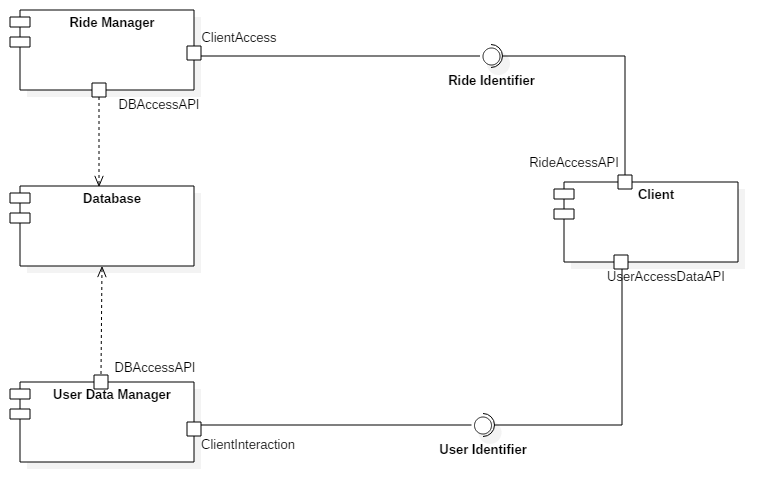
\includegraphics[width=0.9\textwidth]{components/Overview}
	\end{figure}

\subsection{Component View}
	\subsubsection{Client}
		\begin{figure}[h!]
			\centering
			\includegraphics[width=0.9\textwidth]{"components/Client View"}
		\end{figure}
	\subsubsection{Ride Manager}
		\begin{figure}[h!]
			\centering
			\includegraphics[width=0.9\textwidth]{"components/Ride Manager View"}
		\end{figure}

	\subsubsection{Data Manager}
		\begin{figure}[h!]
			\centering
			\includegraphics[width=0.9\textwidth]{"components/User Data Manager View"}
		\end{figure}



\subsection{Deployment View}
	\begin{figure}[h!]
			\centering
			\includegraphics[width=0.9\textwidth]{"components/DeploymentDiagram"}
	\end{figure}

\newpage

\subsection{Runtime View}
	\subsubsection{Sequence Diagram}
		\paragraph{Log In}
			In order to Log In the guest must: \begin{itemize}
				\item Open the service.
				\item Fill the fields with is account data.
				\item Click the Log In button.
			\end{itemize}
			During the Log In the system must check that:\begin{itemize}
				\item All the field are filled with valid data $($The first field must be an email and the second must follow the password validity\askpippo rules$)$.
				\item The email is stored in the database and connected to an account.
				\item The emails-passwords must coincide.
			\end{itemize}
			\newpage
			\begin{figure}[h!]
				\centering
				\includegraphics[width=0.9\textwidth]{"SequenceDiagram/LogIn"}
			\end{figure}
			\newpage

		\paragraph{Instant Call}
			Both the guest and the user must tell their location to call a taxi.\\
			The system must:\begin{itemize}
				\item Check the location given by the guest/user.
				\item Extract from the queue the closest taxi to the given location.
				\item Send the request to the taxi driver.
				\item Confirm the request to the guest/user.
			\end{itemize}
			\begin{figure}[h!]
				\centering
				\includegraphics[width=0.9\textwidth]{"SequenceDiagram/InstantCall"}
			\end{figure}
			\newpage

		\paragraph{Taxi Reservation}
			A user can book a taxi with or without the sharing option by:\begin{enumerate}
				\item Acces the booking {section}.
				\item Fill the requested fields.
			\end{enumerate}
			The system must:\begin{enumerate}
				\item Check the input given by the user.
				\item If Shared Ride must search for a possible ride to join\askpippo.
				\item Update the Database.
			\end{enumerate}

			\begin{figure}[h!]
				\centering
				\includegraphics[width=0.9\textwidth]{"SequenceDiagram/TaxiReservation"}
			\end{figure}
			\newpage

		\paragraph{Edit Boking}
			A user can edit a reservation by:\begin{enumerate}
				\item Selecting the ride to edit from a list.
				\item Edit the ride/cancell the ride.
			\end{enumerate}
			The system must:\begin{enumerate}
				\item Show the user's Booked Ride.
				\item Check if the ride can be edited.
				\item Check the new input given.
				\item If Shared Ride must search for a possible ride to join\askpippo.
				\item Update the Database.
				\end{enumerate}
				\newpage
				\begin{figure}[h!]
					\centering
					\includegraphics[width=0.9\textwidth]{"SequenceDiagram/EditBooked"}
				\end{figure}

\subsection{Component Interfaces}

\subsection{Selected Architectural Styles and Patterns}

\subsection{Further Design Choices}
